\documentclass[11pt,a4paper]{article}

\usepackage[colorlinks=true, linkcolor=black!50!blue, urlcolor=blue, citecolor=blue, anchorcolor=blue]{hyperref}
\usepackage[font=small,labelfont=bf,margin=0mm,labelsep=period,tableposition=top]{caption}
\usepackage[a4paper,top=3cm,bottom=2.5cm,left=2.5cm,right=2.5cm,bindingoffset=0mm]{geometry}

\usepackage{graphicx}
\usepackage{float}
\usepackage{afterpage}
\usepackage{epsfig,cite}
\usepackage{amssymb}
\usepackage{amsmath}
\usepackage{bm}
\usepackage{dsfont}
\usepackage{multirow}
\usepackage{url}
\usepackage{xcolor}
\usepackage{float}
\usepackage{afterpage}
\usepackage{ulem}

\usepackage{url}
\usepackage{hyperref}

\usepackage{multirow,booktabs,multirow}

\bibliographystyle{JHEP}

%%%%%%%%%%%%%%%%%%%%%%%%%%%%%%%%%%%%%%%%%%%%%%%%%%%%%%%%%%%%%

\def\smallfrac#1#2{\hbox{$\frac{#1}{#2}$}}
\newcommand{\be}{\begin{equation}}
\newcommand{\ee}{\end{equation}}
\newcommand{\bea}{\begin{eqnarray}}
\newcommand{\eea}{\end{eqnarray}}
\newcommand{\bi}{\begin{itemize}}
\newcommand{\ei}{\end{itemize}}
\newcommand{\ben}{\begin{enumerate}}
\newcommand{\een}{\end{enumerate}}
\newcommand{\la}{\left\langle}
\newcommand{\ra}{\right\rangle}
\newcommand{\lc}{\left[}
\newcommand{\rc}{\right]}
\newcommand{\lp}{\left(}
\newcommand{\rp}{\right)}
\newcommand{\as}{\alpha_s}
\newcommand{\aq}{\alpha_s\left( Q^2 \right)}
\newcommand{\amz}{\alpha_s\left( M_Z^2 \right)}
\newcommand{\aqq}{\alpha_s \left( Q^2_0 \right)}
\newcommand{\aqz}{\alpha_s \left( Q^2_0 \right)}
\def\toinf#1{\mathrel{\mathop{\sim}\limits_{\scriptscriptstyle
{#1\rightarrow\infty }}}}
\def\tozero#1{\mathrel{\mathop{\sim}\limits_{\scriptscriptstyle
{#1\rightarrow0 }}}}
\def\toone#1{\mathrel{\mathop{\sim}\limits_{\scriptscriptstyle
{#1\rightarrow1 }}}}
\def\frac#1#2{{{#1}\over {#2}}}
\def\gsim{\mathrel{\rlap{\lower4pt\hbox{\hskip1pt$\sim$}}
    \raise1pt\hbox{$>$}}}       
\def\lsim{\mathrel{\rlap{\lower4pt\hbox{\hskip1pt$\sim$}}
    \raise1pt\hbox{$<$}}}       
\newcommand{\mrexp}{\mathrm{exp}}
\newcommand{\dat}{\mathrm{dat}}
\newcommand{\one}{\mathrm{(1)}}
\newcommand{\two}{\mathrm{(2)}}
\newcommand{\art}{\mathrm{art}}
\newcommand{\rep}{\mathrm{rep}}
\newcommand{\net}{\mathrm{net}}
\newcommand{\stopp}{\mathrm{stop}}
\newcommand{\sys}{\mathrm{sys}}
\newcommand{\stat}{\mathrm{stat}}
\newcommand{\diag}{\mathrm{diag}}
\newcommand{\pdf}{\mathrm{pdf}}
\newcommand{\tot}{\mathrm{tot}}
\newcommand{\minn}{\mathrm{min}}
\newcommand{\mut}{\mathrm{mut}}
\newcommand{\partt}{\mathrm{part}}
\newcommand{\dof}{\mathrm{dof}}
\newcommand{\NS}{\mathrm{NS}}
\newcommand{\cov}{\mathrm{cov}}
\newcommand{\gen}{\mathrm{gen}}
\newcommand{\cut}{\mathrm{cut}}
\newcommand{\parr}{\mathrm{par}}
\newcommand{\val}{\mathrm{val}}
\newcommand{\tr}{\mathrm{tr}}
\newcommand{\checkk}{\mathrm{check}}
\newcommand{\reff}{\mathrm{ref}}
\newcommand{\Mll}{M_{ll}}
\newcommand{\extra}{\mathrm{extra}}
\newcommand{\draft}[1]{}
\newcommand{\comment}[1]{{\bf \it  #1}}
\def\beq{\begin{equation}}
\def\eeq{\end{equation}}

% Added by MU 
\def \a{\alpha}
\def \b{\beta}
\def \g{\gamma}
\def \z{\zeta}
\def \t{{\bf T}} % vector of theoretical predictions
\def \c{{\bf c}} % vector of coefficients of theoretical predictions
\def \y{{\bf y}} % vector of experimental data
\def \s{{\bf \sigma}} % experimental covariance matrix
% Added by JR
\def\lapprox{\lower .7ex\hbox{$\;\stackrel{\textstyle <}{\sim}\;$}}
\def\gapprox{\lower .7ex\hbox{$\;\stackrel{\textstyle >}{\sim}\;$}}
\def\half{\smallfrac{1}{2}}
\def\GeV{{\rm GeV}}
\def\TeV{{\rm TeV}}
\def\ap{{a'}}
\def\vp{{v'}}
\def\e{\epsilon}
\def\d{{\rm d}}
\def\calN{{\cal N}}
\def\shat{\hat{s}}
\def\barq{\bar{q}}
\def\qq{q \bar q}
\def\uu{u \bar u}
\def\dd{d \bar d}
\def\pp{p \bar p}
\def\xa{x_{1}}
\def\xb{x_{2}}
\def\xaa{x_{1}^{0}}
\def\xbb{x_{2}^{0}}
\def\smx{\stackrel{x\to 0}{\longrightarrow}}
\def\Li{{\rm Li}}

\numberwithin{equation}{section}
\numberwithin{figure}{section}
\numberwithin{table}{section}

\newcommand{\tmop}[1]{\ensuremath{\operatorname{#1}}}
\newcommand{\tmtextit}[1]{{\itshape{#1}}}
\newcommand{\tmtextrm}[1]{{\rmfamily{#1}}}
\newcommand{\tmtexttt}[1]{{\ttfamily{#1}}}

\usepackage{tabularx}
\newcolumntype{C}[1]{>{\centering\arraybackslash}p{#1}}

\begin{document}
\newgeometry{top=1.5cm,bottom=1.5cm,left=2.5cm,right=2.5cm,bindingoffset=0mm}

\vspace{2cm}

\begin{center}
  {\Large \bf
  Accessing the low-loss region in EELS with machine learning
  }
\vspace{1.4cm}


 Laurien, Luigi, Juan and Sonia\\


\vspace{0.4cm}
       {\it TU Delft and Nikhef
       }

       \vspace{1.0cm}

       {\bf \large Abstract}
       
\end{center}

We use neural networks and Monte Carlo sampling techniques
to provide a model-independent determination of the zero-loss peak
in electron energy-loss spectroscopy (EELS) measurements with faithful uncertainty estimation.

\tableofcontents

\section{Introduction}

Intro to the general problem of low-loss EELS and ZLP background subtraction.

Motivation of the specific materials.

Motivation for the HEP techniques in the context of material sciences.

In this work we will follow the approach pioneering by the NNPDF collaboration~\cite{Ball:2017nwa}.

\part{ZLP in Vacuum}

The first part of this studies is dedicated to the prediction of the shape of the zero loss peak when recorded in vacuum. We construct a generalized N-dimensional model which predicts the ZLP from N arguments. On this basis, we can successfully predict the shape of the ZLP with inter- and extrapolation with respect to each of the input variables. \\

The predicted intensity at any point of the spectrum depends predominantly on the energy loss. We expect the highest intensity at zero loss and the number of counts rapidly decreasing as the energy loss increases. It is common to quantify this decrease in the Full Width Half Maximum (FWHM). Two variables that greatly account for the overall intensity of the ZLP are the exposure time and operating beam current, which both have a positive correlation on the number of counts. \\
Also other factors can account for changing ZLP intensities, such as aperture width and parameters of the electron gun and lenses. These variables could be given as inputs as well, however we expect that these are less relevant than the three input variables mentioned above. Therefore our default model will be built on these three arguments: energy loss, exposure time and beam current. We construct a 3-dimensional model with these continuous inputs and output the ZLP intensity. This model could be extended to an arbitrary dimension N, as long as information on the N input variables is available for training.

\section{The data set (I)}
For the purpose of this study, four different sets of vacuum recorded zero loss peaks are used, each of them measured under a different setting of exposure time and beam current, as listed in table \ref{table:vacuum}. These data sets were recorded with a Titan TEM, equipped with a Skottky field emitter.


\begin{table}[H]
\begin{tabular}{|l|l|l|l|l|l|l|l|l|}
\hline
Set & $t_{exp}$ {[}ms{]} & $E_{beam}$ {[}keV{]} & $N_{files}$ & $N_{dat} / file$ & $dE_{min}$  & $dE_{max}$  & $I_{max}$ & FWHM  \\ \hline
1        & 100                 & 200                  & 15          & 2048               & -0.96              & +8.51               & 739770       & 0.025         \\
2        & 100                 & 60                   & 7           & 2048               & -0.54              & +5.59               & 326483       & 0.022         \\
3        & 10                  & 200                  & 12          & 2048               & -0.18              & +2.97               & 70913        & 0.003         \\
4        & 10                  & 60                   & 6           & 2048               & -0.40              & +4.78               & 30793        & 0.017         \\ \hline
\end{tabular}

\caption{The data sets of the in vacuum recorded zero loss peaks used for this part of the analysis. We show the number of data points ($N_{files}\times N_{dat}$/file), the energetic range, maximum recorded intensity and FWHM of each set of data. FWHM, $dE_{min}$ and $dE_{max}$ are given in eV.}
\label{table:vacuum}
\end{table}

\section{Methodology}

The main ingredients of our road to success will be:
\begin{enumerate}
    \item Data preparation, to set up the raw data for training.
    \item Neural network formulation, where the network architecture, optimization algorithm and loss function are defined.
    \item Minimization, which allows an efficient optimization on the three-dimensional input.
    \item Validation, where the optimal distribution of weights is defined by a stopping criterion and the goodness of the fit is quantified. 
    \item Interpolation and extrapolation, which is the unique selling point of this procedure. 
\end{enumerate}

\subsection{Data preparation}
The four data sets contain spectra that are recorded over a different energy range. As we are only interested in the ZLP region, where the intensity is different from zero, we drop all data that is outside $[-0.1, 0.5]$ eV. This way we capture all the relevant data, discard a big region with zero intensity and we have data for each of the sets over the entire energy range. \\
We then evolve our data from the original scale to a scale at which we can ease the optimization. Unscaled input variables can result in a slow or unstable learning process, whereas unscaled target variables on regression problems can result in exploding gradients causing the learning process to fail \cite{juan}. The energy loss is scaled between [$-1,1$] and all input spectra are scaled between [$0.1, 0.9$], where 0.9 corresponds to the maximum value of the intensity for each separate data set ($I_{max}$, table \ref{table:vacuum}). 

\subsubsection*{Observables}
Central values and errors are calculated for each of the data sets separately, as we expect different outcomes for different exposure time and beam energy. The discretization technique used to assign mean and standard deviation to the data points is Equal Width Discretization (EWD) \cite{ewd}, a simple discretization method that divides the range of observed values for a feature into k equal sized bins. The intervals are computed by 
$\Delta E = (E_{max} - E_{min}) / k$. The value of k is chosen empirically such that the number of bins is high enough to not lose valuable information, but still contains a sufficient number of data points to calculate the uncertainties.\
 Within each energy bin $\Delta E$, the median and variance of all data points within this bin are determined and returned to the original data points. This way, each data point is a vector $[dE, D_i, \sigma_i]$ where dE is the original energy loss; $D_i$ and $\sigma_i$ are the median and std of the bin where this point belongs to. 

\subsubsection*{Monte Carlo sampling}
Error propagation from experimental data to the fit is performed by Monte Carlo sampling of the training data. In a Monte Carlo approach, any statistical property of the function with error - in our case the ZLP - can be derived from a Monte Carlo sample of replicas of the function. By the generation of $N_{rep}$ replicas of the individual training points, a multi-gaussian distribution is obtained centered at $D_i$ with a standard deviation equal to the corresponding error $\sigma_i$. \\
To be precise, given a training data point
\begin{equation}
    Y = Y(dE, D_i,\sigma_i), 
\end{equation} a set of $k= 1,2,..,N_{rep}$ artificial training points is generated by adding a stochastic noise signal on top of the data: 
\begin{equation}
    Y^{(k)} = Y(dE, D_i,\sigma_i) + r^{(k)}\sigma_i.
\end{equation}
The variables $r^{(k)}$ are normally distributed random numbers, such that each element in the Monte Carlo set is a fluctuation around the central value of the experimental data: each replica $k$ contains as many data points as the original set. \\

The value of $N_{rep}$ should be chosen in such a way that the set of replicas models the probability distribution of original training data faithfully. A comparison of the central values and errors of the artificial set with the original data is shown in Fig \ref{mcvacuum} for samples of 100, 500, 1000 and 5000 replicas. The results from a more quantitative comparison can be observed in table \ref{tablemcvacuum}.

\begin{figure}[H]
    \centering 
    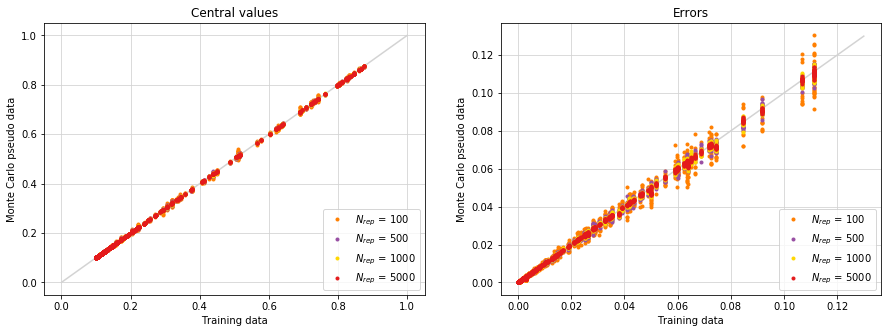
\includegraphics[width=160mm]{plots/Montecarlovacuum.png}
    \caption{Scatter plot of training data vs. Monte Carlo replicas central values (left) and errors (right). }
    \label{mcvacuum}
\end{figure}
\begin{table}[H]
\centering
\begin{tabular}{|l|ll|ll|}
\hline
Nrep & $\textless{\mu}\textgreater{}$ {[}eV{]} & r{[}$\mu${]} & $\textless{\sigma}\textgreater{}$ {[}eV{]} & r{[}$\sigma${]} \\ \hline
100  & 0.10259                           & 0.999919   & 0.63618                                  & 0.996990      \\ \hline
500  & 0.10258                              & 0.999982   & 0.63991                                  & 0.999388      \\ \hline
1000 & 0.10258                              & 0.999991   & 0.64013                                  & 0.999590      \\ \hline
5000 & 0.10258                              & 0.999997   & 0.63980                                  & 0.999776      \\ \hline
\end{tabular}
\caption{Comparison between the artificial and the original central values and errors. $\textless{\mu}\textgreater{}$ and $\textless{\sigma}\textgreater{}$ are the expectation value of the median and errors respectively. The scatter correlation $r$ gives the spread around the straight line. $\textless{\mu^{exp}}\textgreater{}$ = 0.10258, $\textless{\sigma^{exp}}\textgreater{}$ = 0.63970. }
\label{tablemcvacuum}
\end{table}


\subsection{Neural network and fitting strategy}
The neural network architecture that we use is 3-10-15-5-1, enabling deep learning with three hidden layers. This choice is made empirically and it is motivated by the flexibility of the network to overlearn, which is necessary for the post-selection criterion, yet to keep the computation time reasonable. The use of a redundant architecture excludes a priori the bias that an underlearning model would bring forth. 

\subsection{Minimization}

\subsection{Validation}

\subsubsection*{Closure Testing}
In order to validate if the computed error associated to each training point is reasonable, a method called closure testing provides insight \cite{closure}. A closure test ensures that uncertainties introduced by methodology are small compared to the generic experimental errors of the data. A basic requirement for a successful methodology is the ability of generalization, which means that the model works on widely different datasets without the need for manual fine-tuning.\\
The basic idea of closure testing is the following \cite{closure}: we take as general assumed form of the ZLP the smooth fit to the data and we create a set of 'perfect' pseudo data by sampling this smooth function at our data points. Smoothing of the data is realized by application of a Hanning window \cite{hann}, a popular method in signal processing, based on the convolution of a scaled window with the signal. \\
Next, on each 'perfect' data point we impose a gaussian random number with size equal to the corresponding error from the original dataset. If we then train our neural network on these points, given that the pseudo-data are fluctuated on average by one $\sigma$ away from the 'perfect' value, by construction we should find the error function $\chi^2$ of the best fit will be approximately one. Results of the $\chi^2$ values with the closure test can be observed in Fig. \ref{closure1}. These values were obtained with the look-back method discussed in section \textit{ (..nowhere yet..),} which ensures that the final $\chi^2$ is taken at the optimum stopping point, before overlearning sets in.

\begin{figure}[H]
    \centering
    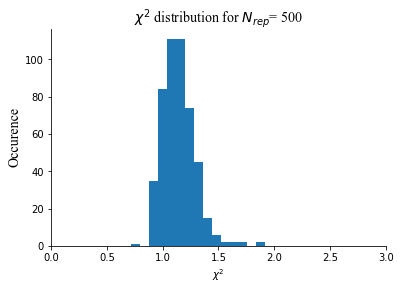
\includegraphics[width=70mm]{plots/chi2.png}
    \caption{Histogram of $\chi^2$ values obtained after training the neural network on 500 sets of artificial data created for closure testing.}
    \label{closure1}
\end{figure}

\subsection{Interpolation and extrapolation}


\newpage
\part{ZLP in Sample}

ZLP in sample, where i) we compare with the vacuum results, ii) we modify the training region to make sure we don't fit the signal from sample, 3) we perform the substraction and look for interesting features in the low-loss spectra

\section{The data set (II)}

The spectra used for the purpose of this study are retrieved from the studies of Miguel Tinoco, Luigi Maduro et. al. \cite{soniamos2} on specific structures of molybdenum disulfide (MoS2). MoS2 is a highly promising material exhibiting a wide range of possible applications for electronic and optical devices. When MoS2 is thinned down to a single monolayer (ML), its indirect band gap switches to a direct band gap of around 1.88 eV \cite{nerl}. \\
A monochromated electron source was used operating at 60 kV, which achieves an energy resolution of around 30 meV. The most-distinctive features of the EELS spectra are two relatively narrow peaks around 1.88 and 2.05 eV, arising from the direct exciton transitions and split by interlayer interactions and spin-orbit coupling. These measurements for the position of the bandgap is consistent with previous studies \cite{nerl, komsa}. The peaks could be revealed after subtraction of a fitted Gaussian curve and a power law to the ZLP and its right-hand tail. \\

An ensemble of electron loss spectra acquired at different positions at the sample is used to construct the training inputs (Fig. \ref{spectra}). As the ZLP is several orders of magnitude bigger than the sample data, the logarithm of the intensity is used to train the model.

The main features of our data sets are summarized in Table \ref{table:spectra}, where we show (...). 

\begin{table}[H]
\centering
\begin{tabular}{|l|l|}
\hline
Property of dataset & Values \\ \hline
1                   & x      \\ \hline
2                   & x      \\ \hline
3                   & x      \\ \hline
4                   & x      \\ \hline
5                   & x      \\ \hline
\end{tabular}
\caption{Table 1}
\label{table:spectra}
\end{table}

\section{Methodology}

The energy loss of the sample data covers a $[-0.3, 8]$ eV range. Since the ZLP feature is several orders of magnitude bigger than the sample features, we take the logarithm of the intensity to train the network. 
 
\subsection{Data processing}
\begin{figure}[H]
    \centering
    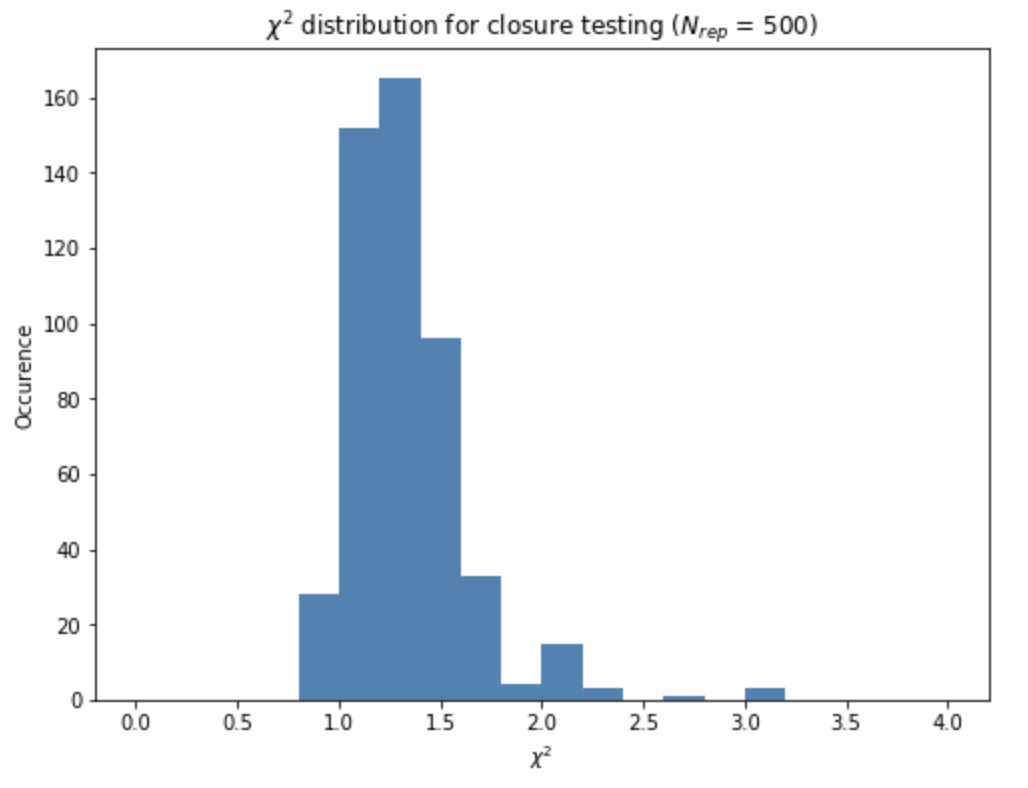
\includegraphics[width=70mm]{plots/closure.png}
    \caption{Histogram of $\chi^2$ values obtained after training the neural network on 500 sets of artificial data created for closure testing.}
    \label{closure2}
\end{figure}

\subsection{Training regions}
It is important to make an informed choice as to the energy range of the input data over which the neural network is trained. Figure \ref{ranges} below is a schematic low-loss spectrum showing five relevant energy ranges \cite{reed}. Region (a) doesn't contain loss electrons and contributions solely come from dark counts in the detector. Range (b) and (c) together form the 'ZLP-region', with the left- and right hand side of the ZLP respectively. Since we make use of a monochromated electron beam, the energy distribution is approximately symmetric around zero and range (c) will be the mirrored version of range (b) until a certain energy limit, which we will call $dE_1$. Range (e) sets in at higher energy loss $dE_2$ and represents the almost pure loss signal, with essentially negligible ZLP contributions. Region (d) is the transition in which the ZLP tail gradually gives way to the loss signal. It is this region that is specifically of interest, as it contains the low-loss features of the sample.  Our objective is to automatically determine the right values for $dE_1$ and $dE_2$ before training the neural network.

\begin{figure}[H]
    \centering
    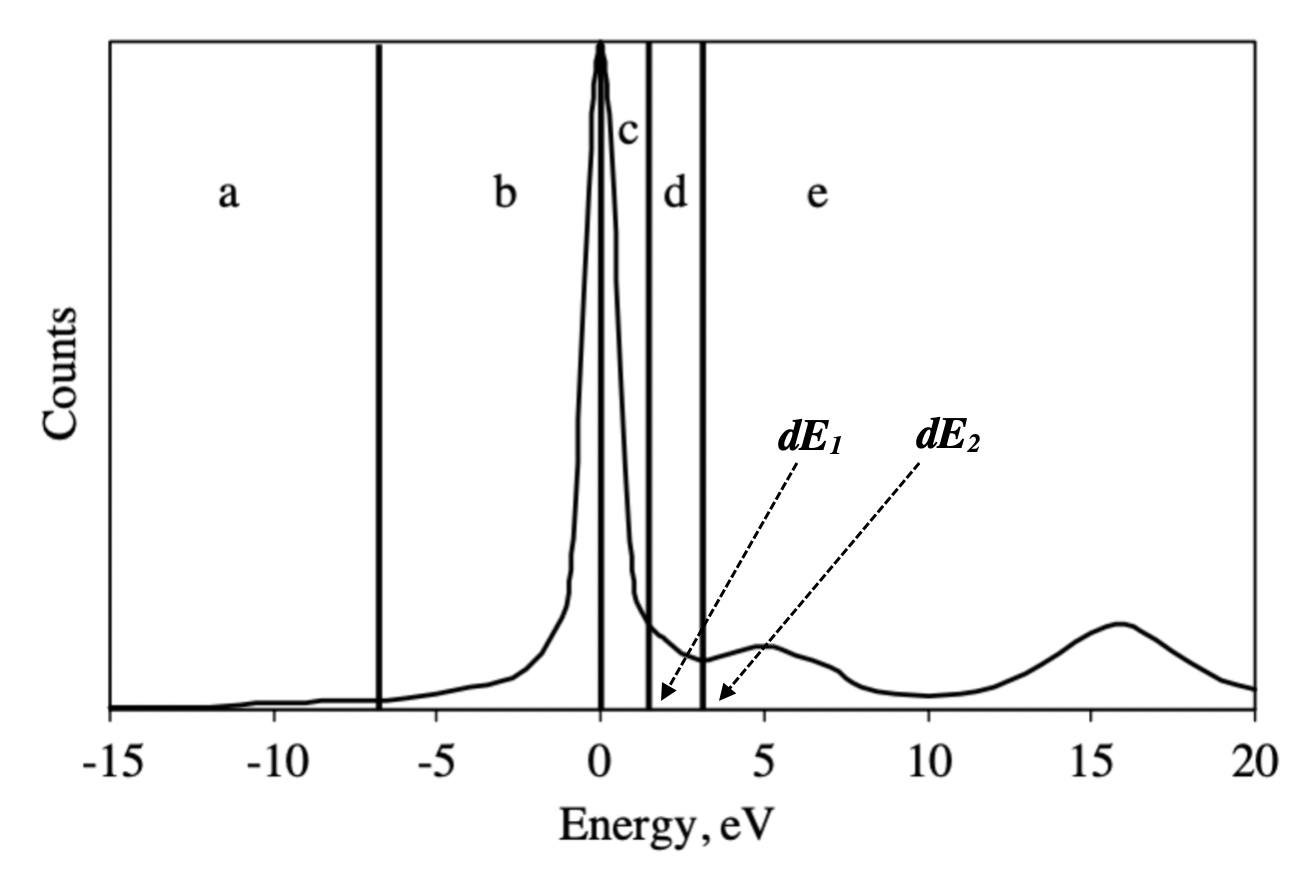
\includegraphics[width=100mm]{plots/ranges.png}
    \caption{Schematic illustration of the relevant energy ranges used in the model}
    \label{ranges}
\end{figure}

Before training, a window is to be applied to the training inputs to an upper boundary $dE_1$, to ensure the network trains on data of the ZLP solely. In order to attain a model that meets $log(I_{ZLP}) \rightarrow 0$ as $dE \rightarrow \infty$, pseudo data is to be added for $E>dE_2$ where the ZLP contribution becomes negligible. The model is trained on data for $E<dE_1$ and $E>dE_2$, the interpolation region $dE_1 < E < dE_2$ contains the predictions of interest. \\

\subsection{Derivatives for preliminary feature identification}

Using first and second derivatives is a feature extraction method to achieve a relatively high accuracy with a low computational complexity. The slope of any function is described by the first derivative, therefore the second derivative is essentially the change in slope, representing the curvature of the signal. This can be useful to determine the boundary from the ZLP to the sample region. \\

In an ideal microscope the electron beam would be perfectly monochromatic, correspondingly the ZLP would appear as a delta function in an EEL spectrum \cite{rafferty}. In practice the ZLP has a finite width defining the energy resolution of the system. At some energy loss the contribution to the sample kicks in and it is at this point that the intensity profile, earlier monotonically decreasing, will have its first local minimum and correspondingly the first derivative will cross zero. It is this point, previously defined as $dE_2$, that marks the transition from the interpolation to the sample region. The first crossing of $\frac{d}{dE}log(I)$ with zero differs slightly between the individual spectra: we take as $dE_2$ the lowest of these, as we can say with certainty that the intensity of the sample has kicked in at the first notice of a local minimum. For this set of data, we find $dE_2$ = $1.468$ eV (Fig. \ref{bound}). 

\begin{figure}[H]
    \centering 
    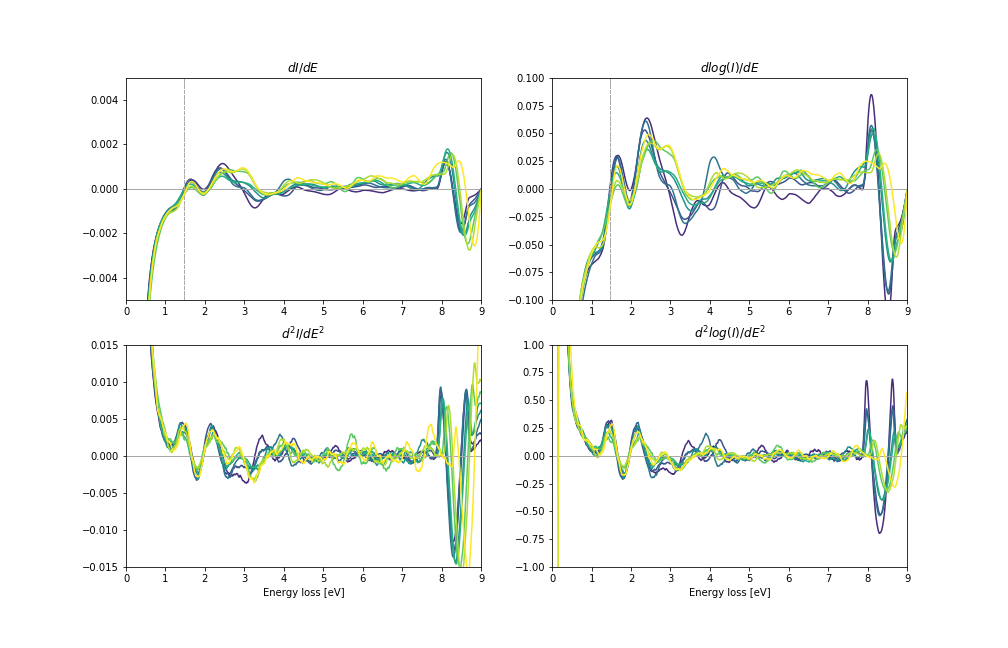
\includegraphics[width=170mm]{plots/derivatives.png}
    \caption{First and second derivatives and log derivatives of the nine experimental spectra. All functions are normalized to the maximum spectrum intensity to make sense of the relative change. The first crossing of the log derivative with zero is \textbf{1.468} eV and marks the transition to the sample region ($dE_2$). Before taking each derivative, smoothing by means of a Hann window \cite{hann} was applied to remove noise and reveal underlying trends. }
    \label{bound}
\end{figure}

From changes in the normalized second derivatives in Fig \ref{bound}, one is able to define significant features appearing in the spectrum. 

By stating that the ideal zero loss peak is symmetric around zero up to energy loss $dE_1$, hypothetically we could determine the value of $dE_2$ by mirroring the left-hand tail to the right side and see when the two significantly start to deviate. In practice however, the ZLP is not symmetric due to various external factors such as astigmatism \cite{astigma} and virtual scattering events \cite{rafferty}, which makes direct reflection of the left-hand tail unfavorable. \\
The value of $dE_1$ will be chosen as $dE_2 / a$, with $a$ a positive integer. The choice of $a$ is empirical and will be cross-validated. \\ 

After the choice on $dE_1$ and $dE_2$, the set of training data (TD) will be prepared taking the following steps:
\begin{enumerate}
    \item Keep only sample data (SD) inside the window [$dE_{min}, dE_1$]
    \item Create pseudo data (PD) with $log(I)$=0 in range [$dE_2, dE_{max}$]
    \item TD = SD + PD
\end{enumerate}

\subsection{Monte Carlo sampling}
The value of $N_{rep}$ should be chosen in such a way that the set of replicas models the probability distribution of original training data faithfully. A comparison of the central values and errors of the artificial set with the original data is shown in Fig \ref{mc} for samples of 100, 500, 1000 and 5000 replicas. The results from a more quantitative comparison can be observed in table \ref{tablemc}.

\begin{figure}[H]
    \centering 
    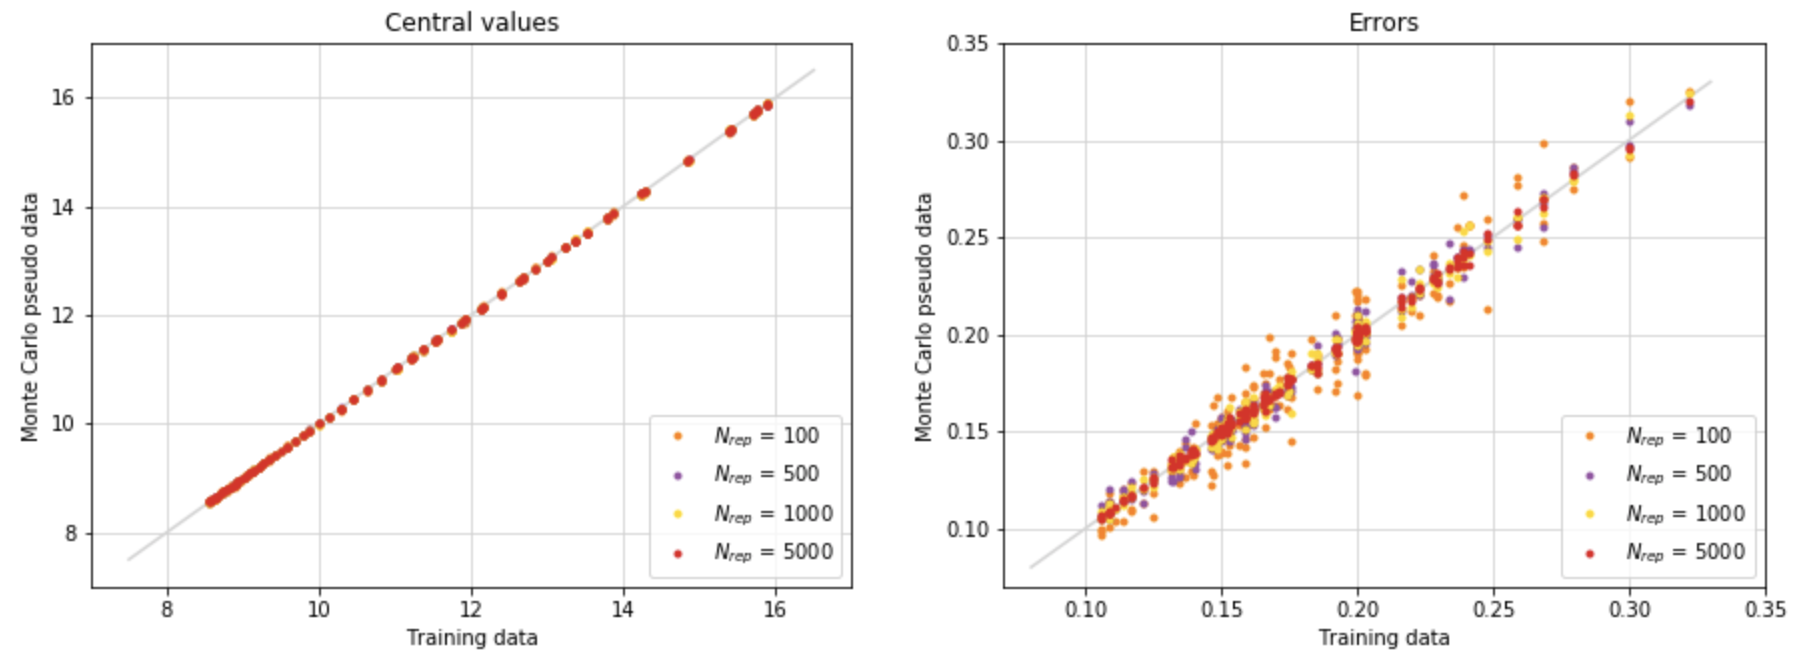
\includegraphics[width=160mm]{plots/MC.png}
    \caption{Scatter plot of training data vs. Monte Carlo replicas central values (left) and errors (right). }
    \label{mc}
\end{figure}

\begin{table}[H]
\centering
\begin{tabular}{|l|ll|ll|}
\hline
Nrep & \textless{}$\mu$\textgreater {[}eV{]} & r{[}$\mu${]} & \textless{}$\sigma$\textgreater {[}eV{]} & r{[}$\sigma${]} \\ \hline
100  & 11.35525                              & 0.99998925   & 0.17783                                  & 0.96617604      \\ \hline
500  & 11.35693                              & 0.99999808   & 0.17799                                  & 0.99172921      \\ \hline
1000 & 11.35578                              & 0.99999894   & 0.17812                                  & 0.99527003      \\ \hline
5000 & 11.35643                              & 0.99999979   & 0.17807                                  & 0.99920997      \\ \hline
\end{tabular}
\caption{Comparison between the artificial and the original central values and errors. $<\mu>$ and $<\sigma>$ are the expectation value of the median and errors respectively. The scatter correlation $r$ gives the spread around the straight line. $<\mu^{(exp)}>$ = 11.35623, $<\sigma^{(exp)}>$ = 0.17805. }
\label{tablemc}
\end{table}

\subsection{ZLP subtraction}
Repetitive training of the neural network on each set of MC pseudo data yields a prediction that is distributed with a mean and std corresponding to the mean and error of the original training set. For each replica, the predicted ZLP is subtracted from the individual original spectra to obtain one set of subtractions. Repeating this procedure yields a collection of $N_{rep}$ subtractions for each original spectrum, over which statistical properties such as median and variance can be calculated. \\

Direct subtraction of the predicted ZLP on each of the original spectra doesn't yield a physical result, as the intensity of the samples in range (a)-(c) (Fig. \ref{ranges}) doesn't coincide between themselves and the predicted ZLP. In order for the subtracted spectrum to make physical sense, we impose that the ZLP to be subtracted will be a smooth transition from the exact replicate of the ZLP in region (a)-(c) to the prediction from the neural network in region (d),(e). This way, we keep only the prediction of the region of our interest. The smooth matching of the ZLP will be the following:
\begin{align}
 dE &< dE_0          &   I_{ZLP}^{(k)} &= I_{orig}\\
 dE_0 &< dE < dE_1   &  I_{ZLP}^{(k)} &= I_{NN}^{(k)} \times  \left( 1 - \exp(-(dE - dE_1)^2/\delta^2)\right) \\
 dE_1 &< dE < 10 \cdot dE_2 &  I_{ZLP}^{(k)} &= I_{NN}^{(k)}\\
 dE &> 10 \cdot dE_2 &   I_{ZLP}^{(k)} &= 0
\end{align}
Here $dE_0$ is the start of the smooth transition from ZLP to NN region given by eq. $(5.4)$, with $dE_0<dE_1$  and $\delta \ll |dE_0 - dE_1|$. 

\begin{figure}[H]
    \centering
    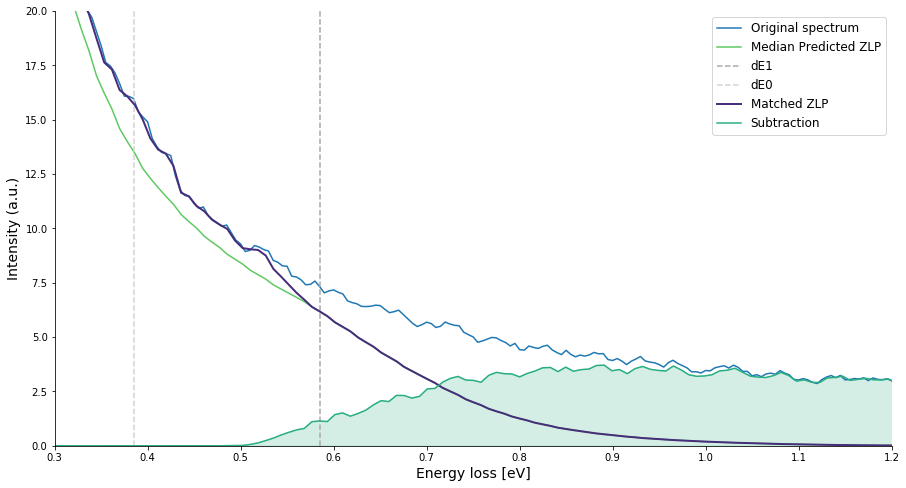
\includegraphics[width=120mm]{plots/matching.png}
    \caption{Representation of the smooth transition from $I_{ZLP} = I_{orig}$ for $dE<dE_0$ to$I_{ZLP} = I_{NN}$ for $dE>dE_1$. }
    \label{fig:my_label}
\end{figure}

\subsection{Ratios for eventual feature identification}

In order to compare the level of desired signal from the sample to the level of the modeled ZLP tail, we define two working definitions, first of which the sample-to-peak ratio (SPR):

\begin{equation}
    SPR_{i}^{(k)} = \frac{I_{orig, i} - I_{ZLP}^{(k)}}{I_{ZLP}^{(k)}}
\end{equation}
where $i$ is the number of the original spectra, $k$ runs over the number of replicas ($k=1,..,N_{rep}$) and $I_{ZLP}$ is the predicted ZLP for that replica. By summing over all replicas, the median and error of $SPR_i$ give a measure for the contribution of the sample to the total intensity profile at any point over the spectrum. \\

To verify the significance of the SPR, we introduce the sample-to-error ratio (SER):
\begin{equation}
    SER_{i}^{(k)} = \frac{I_{orig, i} - I_{ZLP}^{(k)}}{\sigma_{ZLP}}
\end{equation}
where $\sigma_{ZLP}$ is the error of the predicted ZLP calculated over all replicas. 
If the SER is bigger than a certain treshold (e.g. 5), the signal from the sample significantly excesses the background error. \\
Using the definitions of SPR and SER for each original spectrum, it is convenient to define three regions: the 'ZLP region' where $SPR \rightarrow0$, corresponding to region (a)-(c) (Fig. \ref{ranges}) ending at $dE_1$, the 'interpolation region' (d) between $[dE_1, dE_2]$ and the 'sample region' (e) where $SPR\rightarrow\infty$ as $I_{ZLP}\rightarrow0$.


\section{Results}
Here we present the main results of this paper

\section{Summary and outlook}
....

\section{Appendix}


\begin{figure}[H]
    \centering
    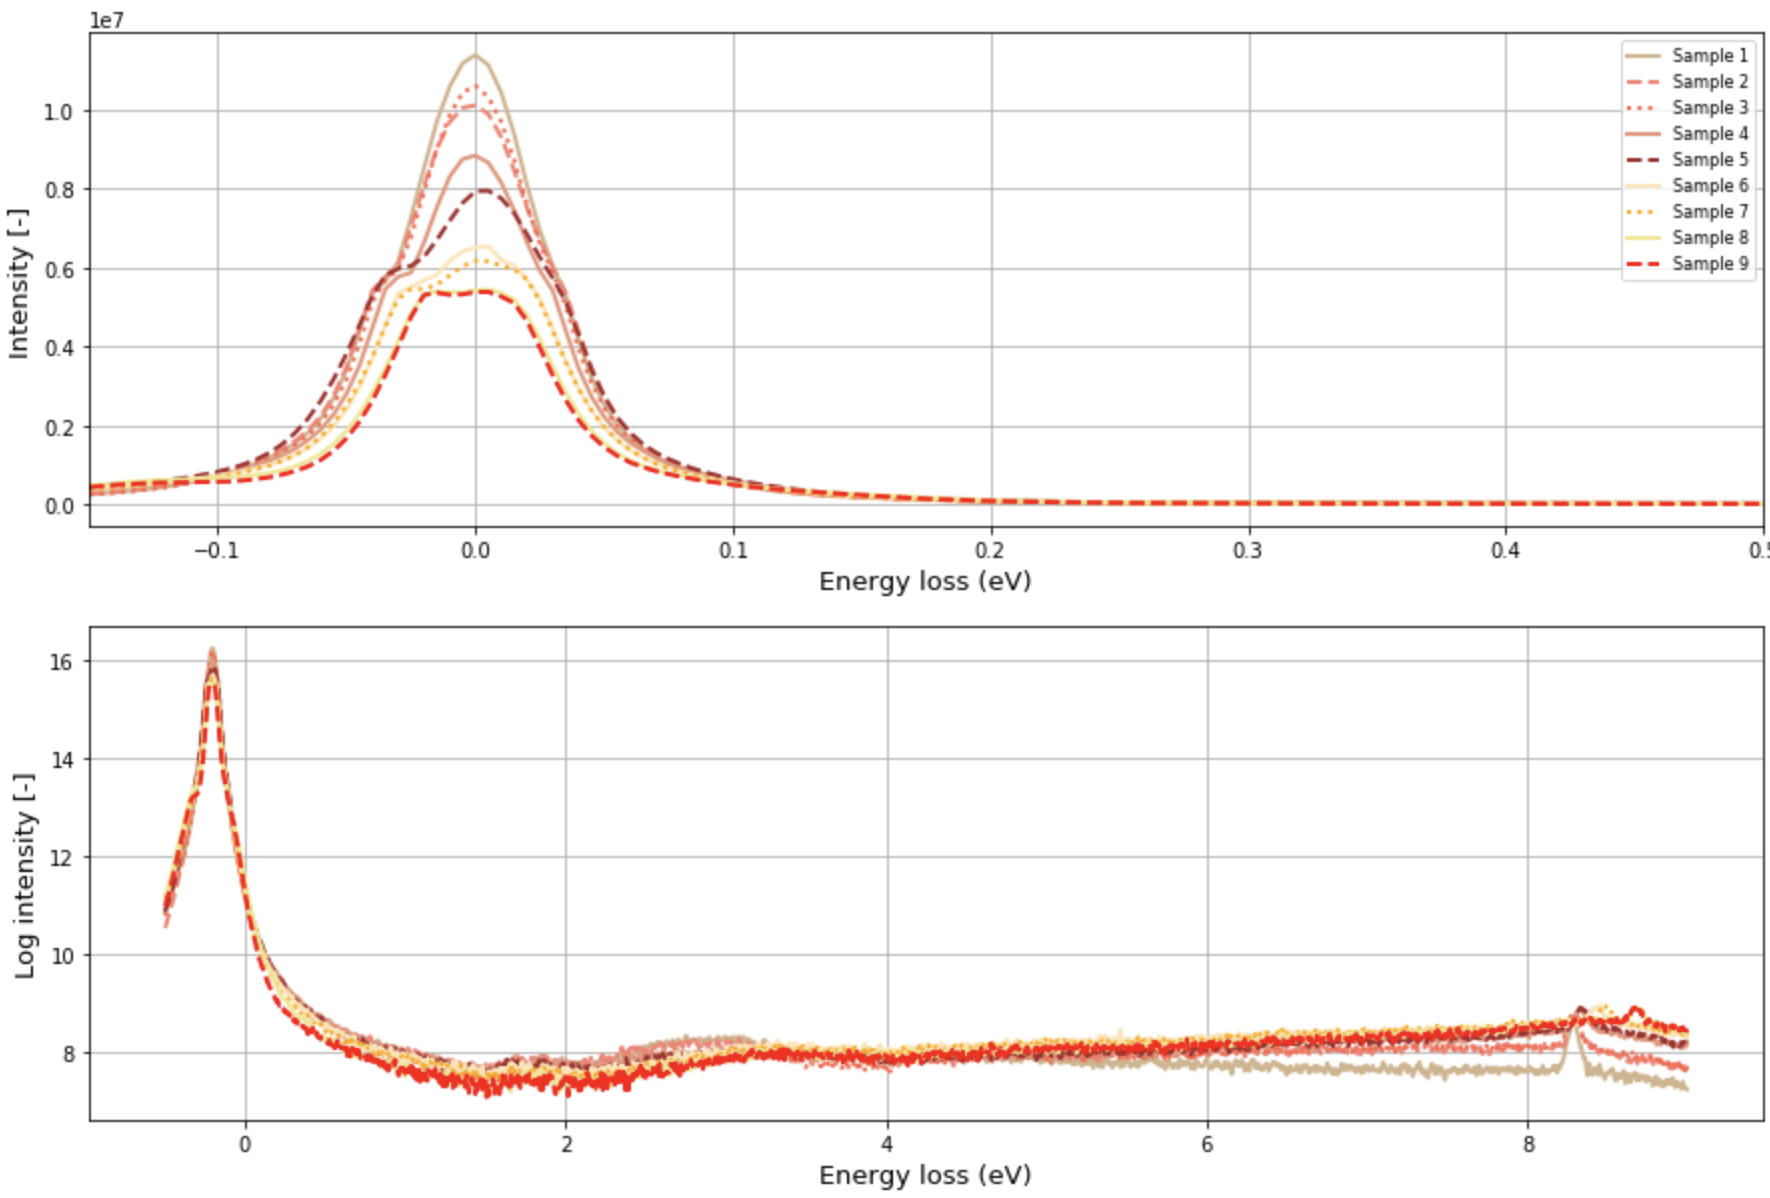
\includegraphics[width=130mm]{plots/spectrum.png}
    \caption{Energy electron loss spectra taken at nine different positions on a sample of MoS2. Up: original intensity. Below: logarithmic intensity. Retrieved from \cite{soniamos2}. }
    \label{spectra}
\end{figure}


\begin{figure}[H]
    \centering
    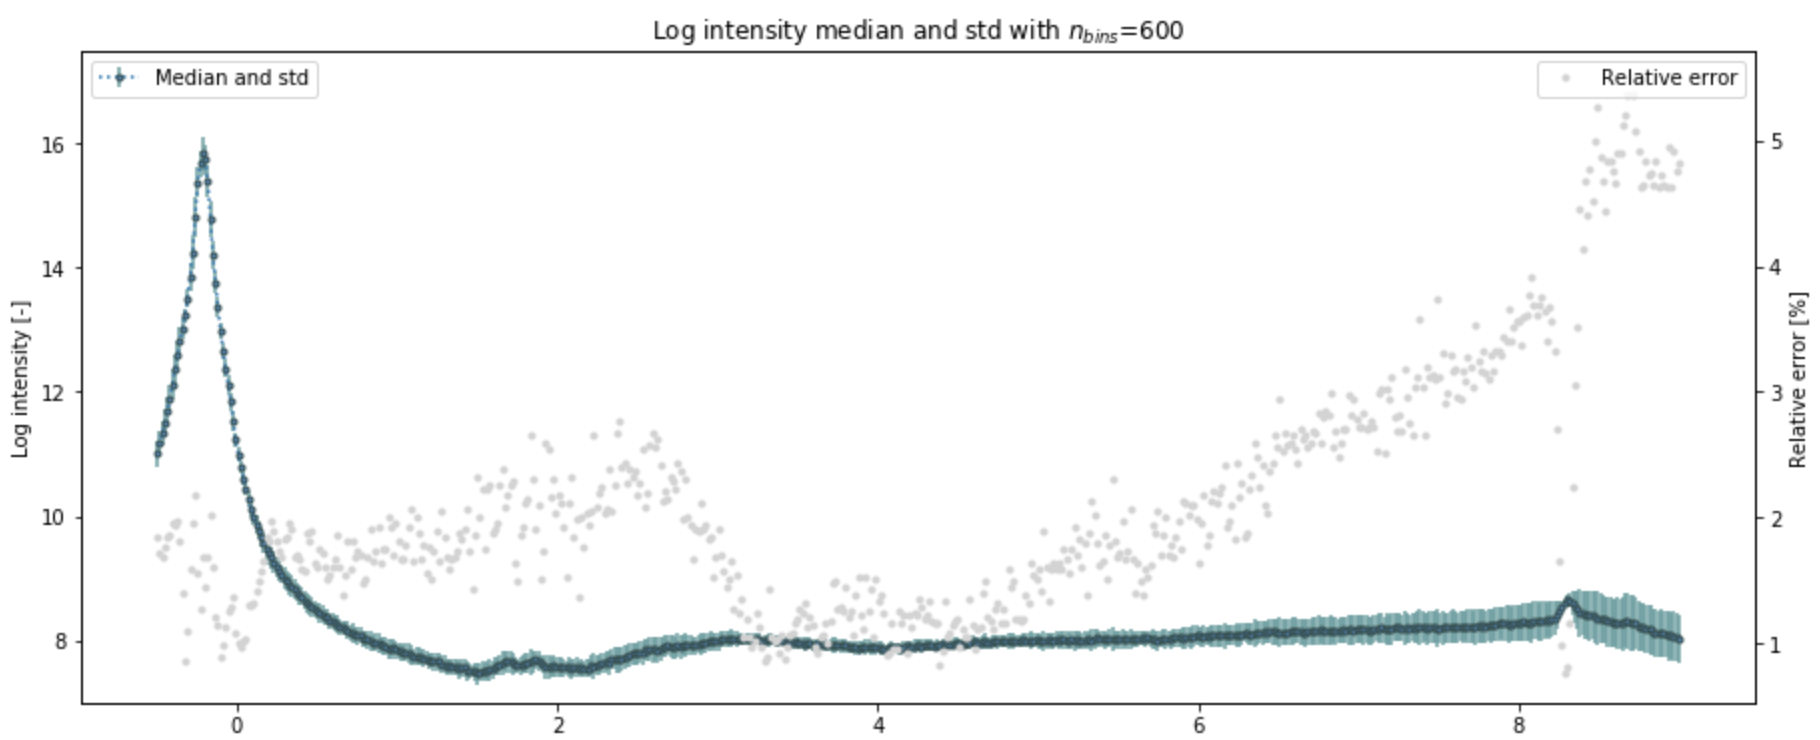
\includegraphics[width=155mm]{plots/ewd.png}
    \caption{Log intensity profile of the sample data after applying EWD with $n_{bins}$=600.}
    \label{ranges}
\end{figure}


\bibliography{main}
\end{document}